\documentclass[
	% -- opções do artigo       -- %
	12pt,				% tamanho da fonte
	a4paper,			% tamanho do papel.
	% -- opções do pacote babel -- %
	english,			% idioma adicional para hifenização
	brazil				% o último idioma é o principal do documento
	]{article}
\usepackage[utf8]{inputenc}
\usepackage{geometry}
\usepackage{mathptmx}           % Utiliza times como fonte
\usepackage[T1]{fontenc}		% Selecao de codigos de fonte.
\usepackage[utf8]{inputenc}		% Codificacao do documento (conversão automática dos acentos)
\usepackage{microtype} 			% para melhorias de justificação
\usepackage{titlesec}           % para editar titulos, capitulos e subcapitulos
\usepackage{fancyhdr}           % para editar o footer e header
\usepackage{indentfirst}        % para identar primeiro paragrafo apos seçao
\usepackage{ragged2e}
\usepackage{array}           

% Pacotes para referências em ABNT2
\usepackage[brazilian]{backref}	 
\usepackage[alf]{abntex2cite}

% Para formatar caption, transformar Figure em Figura em negrito
\usepackage[labelsep=endash, font=small,labelfont=bf]{caption}
% Para adicionar texto abaixo de imagem conforme ABNT
\usepackage[capposition=top, font=small]{floatrow}
\renewcommand{\figurename}{Figura}

% Pacote para imagens
\usepackage{graphicx}
\graphicspath{ {./pics/} }

% Para gerar numero de seçao nas refs
\usepackage[numbib]{tocbibind}

%--------------------------------- %
% Formatacao de Cabeçalho e Rodapé %
%--------------------------------- %
\pagestyle{fancy} % Turn on the style
\fancyhf{} % sets both header and footer to nothing
\renewcommand{\headrulewidth}{0pt}
\fancyfoot[R]{\thepage}

%--------------------------------- %
% Formatacao de Seção e Subseção   %
%--------------------------------- %
\titleformat{\section}{\normalfont\normalsize\bfseries}{\thesection}{1em}{}
\titleformat{\subsection}{\normalfont\normalsize\bfseries}{\thesubsection}{1em}{}
 
% distancia entre linhas
\renewcommand{\baselinestretch}{1.5}

%--------------------------------- %
% Redefinicao do Sumario para      % 
% gerar heading no centro          %
%--------------------------------- %
\makeatletter
\renewcommand{\contentsname}{Sumário}
\renewcommand\tableofcontents{%
  \null\hfill\textbf{\Large\contentsname}\hfill\null\par
  \@mkboth{\MakeUppercase\contentsname}{\MakeUppercase\contentsname}%
  \@starttoc{toc}%
}
\makeatother

%--------------------------------- %
% Formatacao de Margens FAPESP     %
%--------------------------------- %
\geometry{
    top=2.5cm,
    left=3cm,
    right=1.5cm,
    bottom=2.5cm
 }
 

\begin{document}

\begin{titlepage}

    \begin{center}
        \vspace{1cm}
        
        % Modificar width se necessário %
        \includegraphics[width=0.1\textwidth]{/logo_instituicao.png}  
         
        \MakeUppercase{Nome Universidade} 
        \\
        \MakeUppercase{Nome Departamento}
        
        \vspace{2cm}
        \LARGE
        \textbf{Titulo do Projeto}
    \end{center}
    
    \vspace{2cm}
    
    \begin{tabular}{>{\raggedright}p{0.5\linewidth}}
        \begin{center}
            % Modificar width se necessário %
            \includegraphics[width=0.1\textwidth]{/logo_fapesp.png} 
        \end{center}
        Projeto \justifying{apresentado à Fundação de Amparo à Pesquisa do Estado de São Paulo – FAPESP para solicitação de bolsa de Mestrado} 
    \end{tabular}
    
    \vspace{2cm}
    
    \vspace{1cm}
    \begin{tabular}{>{\raggedright}p{0.5\linewidth}}
        Candidato: \textbf{Nome do Candidato} 
        \\
        Orientador: \textbf{Nome do orientador}
    \end{tabular}
    

    \begin{center}
        \vfill
        Cidade - Estado
        \\
        Ano
        \vspace{0.8cm}
    \end{center}
    
\end{titlepage}

\newpage

\tableofcontents
\addtocontents{toc}{\protect\thispagestyle{empty}}

\newpage

%--------------------------------- %
% Seção  Exemplo                   %
%--------------------------------- %
\section{Seção  Exemplo}

%--------------------------------- %
% Subseção Exemplo                 %
%--------------------------------- %
\subsection{Subseção Exemplo}
\label{sec:exemp1}

\par Seu texto aqui.Utilizar \texttt{cite} para citacao direta ABNT e \texttt{citeonline} para citação indireta ABNT

\par $Formula$ 

\begin{figure*}[htp]
    \centering
    \caption{Exemplo Figuras}
    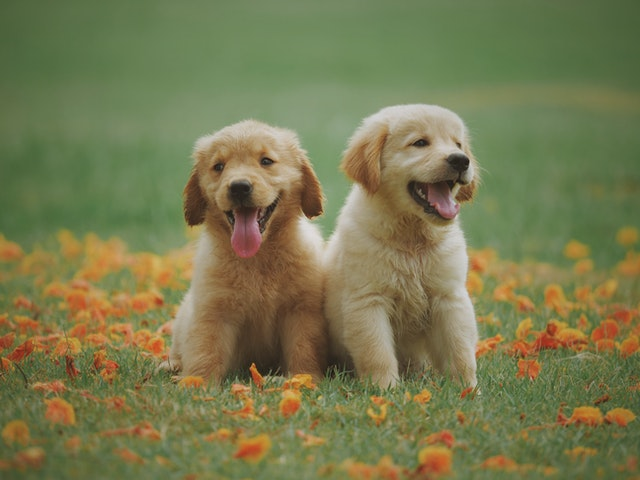
\includegraphics[width=10cm]{/figura.png}
    \floatfoot{Fonte: fonte da imagem}
    \label{fig:kg}
\end{figure*}



%--------------------------------- %
% Seção de Referências             %
%--------------------------------- %
\renewcommand{\refname}{Referencial Bibliográfico}
\bibliography{refs}
    


\end{document}
